
% utf-8 ru, unix eolns
\documentclass[12pt,a4paper,oneside]{extarticle}
    \righthyphenmin=2 %минимально переносится 2 символа %%%
    \sloppy

% Рукопись оформлена в соответствии с правилами оформления 
% электронной версии авторского оригинала, 
% принятыми в Издательстве МГТУ им. Н.Э. Баумана.

\usepackage{geometry} % А4, примерно 28-31 строк(а) на странице 
    \geometry{paper=a4paper}
    \geometry{includehead=false} % Нет верх. колонтитула
    \geometry{includefoot=true}  % Есть номер страницы
    \geometry{bindingoffset=0mm} % Переплет    : 0  мм
    \geometry{top=20mm}          % Поле верхнее: 20 мм
    \geometry{bottom=25mm}       % Поле нижнее : 25 мм 
    \geometry{left=25mm}         % Поле левое  : 25 мм
    \geometry{right=25mm}        % Поле правое : 25 мм
    \geometry{headsep=10mm}  % От края до верх. колонтитула: 10 мм
    \geometry{footskip=20mm} % От края до нижн. колонтитула: 20 мм 

\usepackage{cmap}
\usepackage[T2A]{fontenc} 
\usepackage[utf8x]{inputenc}
\usepackage[english,russian]{babel}
\usepackage{misccorr}

\usepackage{amsmath}
\usepackage{amsfonts}
\usepackage{amssymb}

%\usepackage{cm-super} %человеческий рендер русских шрифтов

\setlength{\parindent}{1.25cm}  % Абзацный отступ: 1,25 см
\usepackage{indentfirst}        % 1-й абзац имеет отступ

\usepackage{setspace}   

\onehalfspacing % Полуторный интервал между строками

\makeatletter
\renewcommand{\@oddfoot }{\hfil\thepage\hfil} % Номер стр.
\renewcommand{\@evenfoot}{\hfil\thepage\hfil} % Номер стр.
\renewcommand{\@oddhead }{} % Нет верх. колонтитула
\renewcommand{\@evenhead}{} % Нет верх. колонтитула
\makeatother

\usepackage{fancyvrb}


\usepackage[pdftex]{graphicx}  % поддержка картинок для пдф
\graphicspath{ {./pictures/} }
\usepackage{rotating}
%\DeclareGraphicsExtensions{.jpg,.png}




\renewcommand{\labelenumi}{\theenumi.} %меняет вид нумерованного списка

\usepackage{perpage} %нумерация сносок 
\MakePerPage{footnote}

\usepackage[all]{xy} %поддержка графов

\usepackage{listings} %листинги
\renewcommand{\lstlistingname}{Листинг}
\lstset{
  basicstyle=\tiny,
  breaklines=true
  }


\usepackage{url}


\usepackage{tikz} %для рисования графиков
\usepackage{pgfplots}

\usepackage{gensymb}

\usepackage{ccaption}%изменяет подпись к рисунку
\makeatletter 
\renewcommand{\fnum@figure}[1]{Рисунок~\thefigure~---~\sffamily}
\makeatother

\begin{document}
\pgfplotsset{compat=1.8}

\thispagestyle{empty}
\newpage
{
\centering


\textbf{
МОСКОВСКИЙ ГОСУДАРСТВЕННЫЙ ТЕХНИЧЕСКИЙ УНИВЕРСИТЕТ ИМЕНИ Н. Э. БАУМАНА \\
Факультет информатики и систем управления \\
Кафедра теоретической информатики и компьютерных технологий}
\bigskip
\bigskip
\bigskip
\bigskip
\bigskip
\bigskip
\bigskip

\vfill


Лабораторная работа №1 \\
по курсу <<Математическое моделирование>>

\bigskip

{\large <<Установление степенной взаимосвязи между двумя выборками>>}
\bigskip

\vfill



\hfill\parbox{4cm} {
Выполнил:\\
студент ИУ9-111 \hfill \\
Выборнов А. И.\hfill \medskip\\
Руководитель:\\
Домрачева А. Б.\hfill
}


\vspace{\fill}

Москва \number\year
\clearpage
}



\clearpage


\section{Постановка задачи}
    Имеются две выборки. Одна задаёт курс рубля по отношению к доллару в промежуток от 03.01.2012 до 26.10.2015, другая задаёт курс нефти марки Brent в долларах за такой же промежуток. Необходимо установить взаимосвязь (параметры степенной зависимости) между этими двумя выборками.

    В таблицах~\ref{tabular:data} и ~\ref{tabular:data1} приведён пример входных данных, используемых при решении задачи.
    \begin{table}[ht!]
        \caption{Курс рубля к доллару за один месяц}
        \centering
        \label{tabular:data}
        \small
        \begin{tabular}{|c|c|}
            \hline
            Дата  & Курс рубля к доллару \\ \hline
            30.12.2014 & 56.5828 \\ \hline
            29.12.2014 & 56.1414 \\ \hline
            29.12.2014 & 56.1414 \\ \hline
            26.12.2014 & 52.8703 \\ \hline
            25.12.2014 & 53.7621 \\ \hline
            24.12.2014 & 54.5074 \\ \hline
            23.12.2014 & 54.5440 \\ \hline
            22.12.2014 & 56.2232 \\ \hline
            19.12.2014 & 60.2196 \\ \hline
            18.12.2014 & 60.6779 \\ \hline
            17.12.2014 & 67.4157 \\ \hline
            16.12.2014 & 65.1875 \\ \hline
            15.12.2014 & 59.0116 \\ \hline
            12.12.2014 & 57.2028 \\ \hline
            11.12.2014 & 54.9608 \\ \hline
            10.12.2014 & 54.3048 \\ \hline
            09.12.2014 & 54.1850 \\ \hline
            08.12.2014 & 53.4806 \\ \hline
            05.12.2014 & 53.4319 \\ \hline
            04.12.2014 & 53.1632 \\ \hline
            03.12.2014 & 53.9835 \\ \hline
            02.12.2014 & 51.6665 \\ \hline
            01.12.2014 & 52.2054 \\ \hline
        \end{tabular}
    \end{table}

    \begin{table}[ht!]
        \caption{Курс нефти марки Brent в долларах за один месяц}
        \centering
        \label{tabular:data1}
        \small

        \begin{tabular}{|c|c|}
            \hline
            Дата & Курс нефти марки Brent в долларах \\ \hline
            31.12.2014 & 57.33 \\ \hline 
            30.12.2014 & 57.90 \\ \hline 
            29.12.2014 & 57.88 \\ \hline 
            28.12.2014 & 59.85 \\ \hline 
            26.12.2014 & 59.45 \\ \hline 
            24.12.2014 & 60.24 \\ \hline 
            23.12.2014 & 61.69 \\ \hline 
            22.12.2014 & 60.11 \\ \hline 
            21.12.2014 & 61.56 \\ \hline 
            19.12.2014 & 61.38 \\ \hline 
            18.12.2014 & 59.27 \\ \hline 
            17.12.2014 & 61.18 \\ \hline 
            16.12.2014 & 59.86 \\ \hline 
            15.12.2014 & 61.06 \\ \hline 
            14.12.2014 & 61.08 \\ \hline 
            12.12.2014 & 61.85 \\ \hline 
            11.12.2014 & 63.68 \\ \hline 
            10.12.2014 & 64.24 \\ \hline 
            09.12.2014 & 66.84 \\ \hline 
            08.12.2014 & 66.19 \\ \hline 
            07.12.2014 & 67.97 \\ \hline 
            05.12.2014 & 69.07 \\ \hline 
            04.12.2014 & 69.64 \\ \hline 
            03.12.2014 & 69.92 \\ \hline 
            02.12.2014 & 70.54 \\ \hline 
            01.12.2014 & 72.54 \\ \hline 
        \end{tabular}
    \end{table}
\section{Реализация}

\section{Ход выполнения}

    Пусть выборка $\xi_1$ задаёт курс рубля, а выборка $\xi_2$ --- стоимость нефти.
    Необходимо установить степенную завиисимость между двумя выборками: $$\xi_1=\alpha\xi_2^{\beta}.$$

    Преобразуем степенную зависимость, прологарифмировав обе части равенства, получим: $$ln \xi_1 = ln \alpha + \beta ln \xi_2~~~ (1).$$


    %Рассматриваем новые случайные величины $ln \xi_1$ и $ln \xi_2$
       
    Представив выборку $\xi_1 = \{x_1, . . . , x_n\}$, а выборку $\xi_2 = \{y_1, . . . , y_m\}$, получим:
    $$\frac{1}{n}\sum_{i=1}^{n} ln x_i = ln \alpha + \frac{\beta}{n} \sum_{i=1}^{n} ln y_i,$$
    $$\alpha = e^{M_1-\beta M_2}.$$

    Аналогичным образом найдём параметр $\beta$, взяв дисперсию от обеих частей равенста 1:

    $$D (ln \xi_1) = D(ln \alpha + \beta ln \xi_2),$$
    $$D (ln \xi_1) = D(ln \alpha) + D(\beta ln \xi_2) + 2 cov(ln \alpha, \beta ln \xi_2),$$
    $$D (ln \xi_1) = \beta^2 D(ln \xi_2), $$
    $$\beta = \sqrt{\frac{D (ln \xi_1)}{D (ln \xi_2)}}$$

    Было написано приложение, позволяющее получать по выборкам коэффициется $\alpha$ и $\beta$. Результаты работы показаны на рисунке~\ref{pic:tree} в виде зависимости коэффициентов $\alpha$ и $\beta$ от объёмов выборки. Из рисунка видно, что коэффициенты быстро стабилизируются, что указывает на наличие высокой корреляции между двумя выборками. А также, что существует нелинейная зависимость между двумя исходными выборками вида: $$\xi_1 = 0.78*\xi_2^{0.69}.$$ 

    \begin{figure}[h!]
        \center
        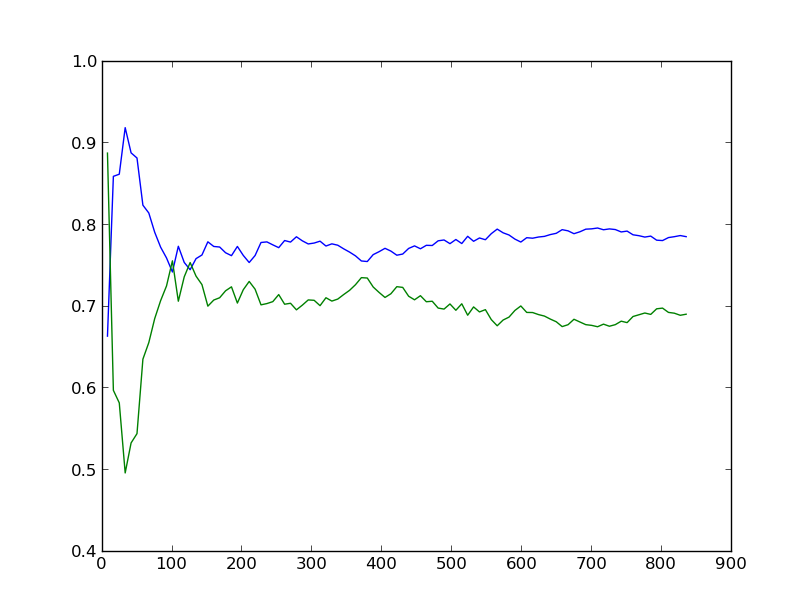
\includegraphics[scale=0.7]{../model.png}
        \caption{Зависимость коэффициентов $\alpha$ (синий график) и $\beta$ (зелёный график) от объёма выборки}
        \label{pic:tree}
    \end{figure}

    С помощью критерия Колмогорова-Смиронова изучим влияние размера обучающей выборки на качество построенное модели. 

    Входные данные делились на две части: обучающая и контрольная выборка. То есть чем больше обучающая, тем меньше контрольная и наоборот.

    На рисунке~\ref{pic:test} показана зависимость качества полученной модели от размера обучающей выборки (чем значение функции меньше, тем более высокое качество модели). Из рисунка видно, что с увеличением размера обучающей выборки качество долгое время остаётся неизменным, а затем резко возрастает. Повышение качества при большом объёме обучающей выборки, предположительно связано, с малым количеством элементов, которые попали в контрольную выборку.

    \begin{figure}[h!]
        \center
        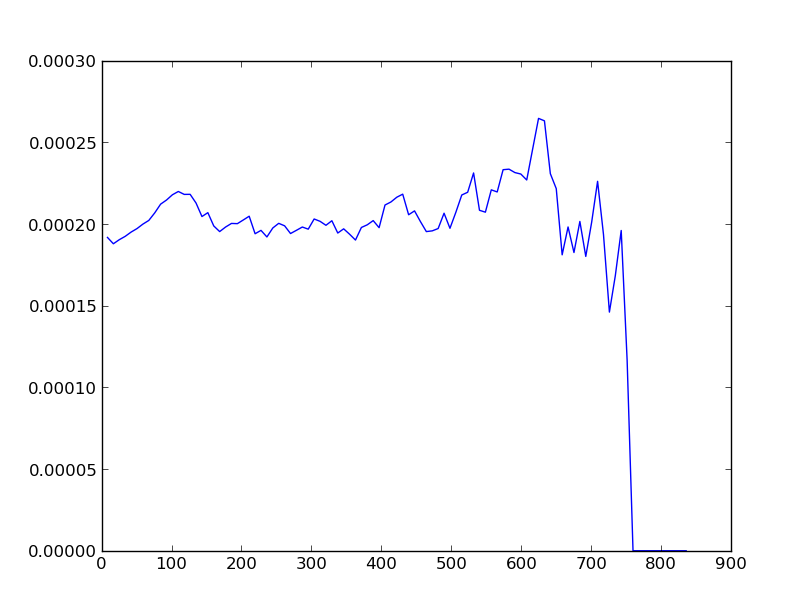
\includegraphics[scale=0.7]{../kolmogorov.png}
        \caption{Зависимость качества построенной модели от размера обучающей выборки (чем значение меньше, тем качество выше)}
        \label{pic:test}
    \end{figure}

\end{document}
